\subsubsection{Thích ứng khi xoay màn hình và thay đổi kích thước}
Android chọn các biến thể XML theo hướng màn hình và kích thước nhỏ nhất, gồm \texttt{layout-land} và \texttt{sw600dp}. Trên tablet ngang, Trang chủ chuyển vùng tìm kiếm sang cột bên trái và hiển thị phòng theo grid; kênh Host tách vùng chọn phòng/tòa nhà khỏi danh sách. Hình~\ref{fig:adaptive-user-host} minh họa hai bố cục này. Các vùng dữ liệu cuộn độc lập để nút và nội dung không bị thanh điều hướng che khuất.

\begin{figure}[H]\centering
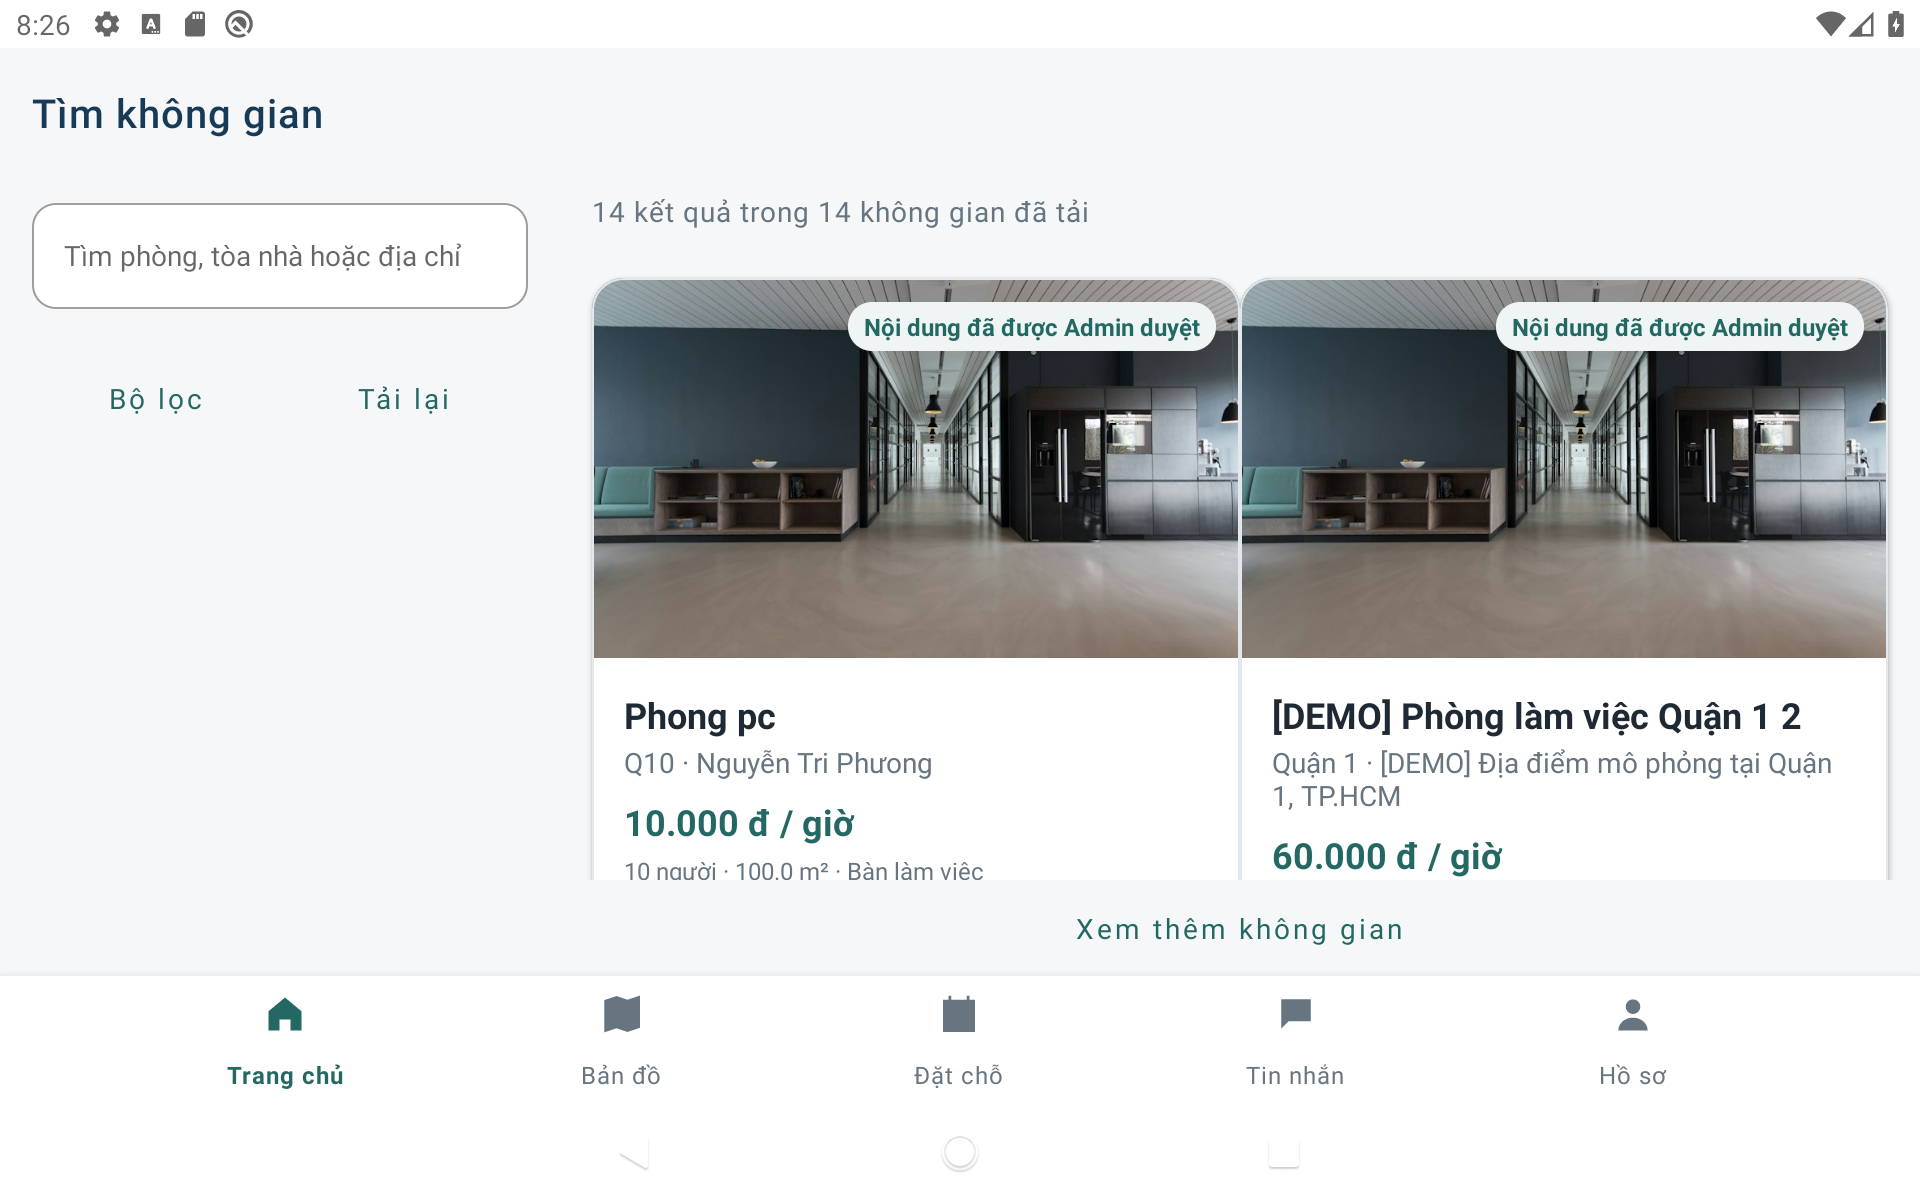
\includegraphics[width=0.94\linewidth]{chapter5/members/user-tablet-home-landscape.png}\\[-1mm]
{\small (a) Trang chủ ở chế độ thuê}
\par\medskip
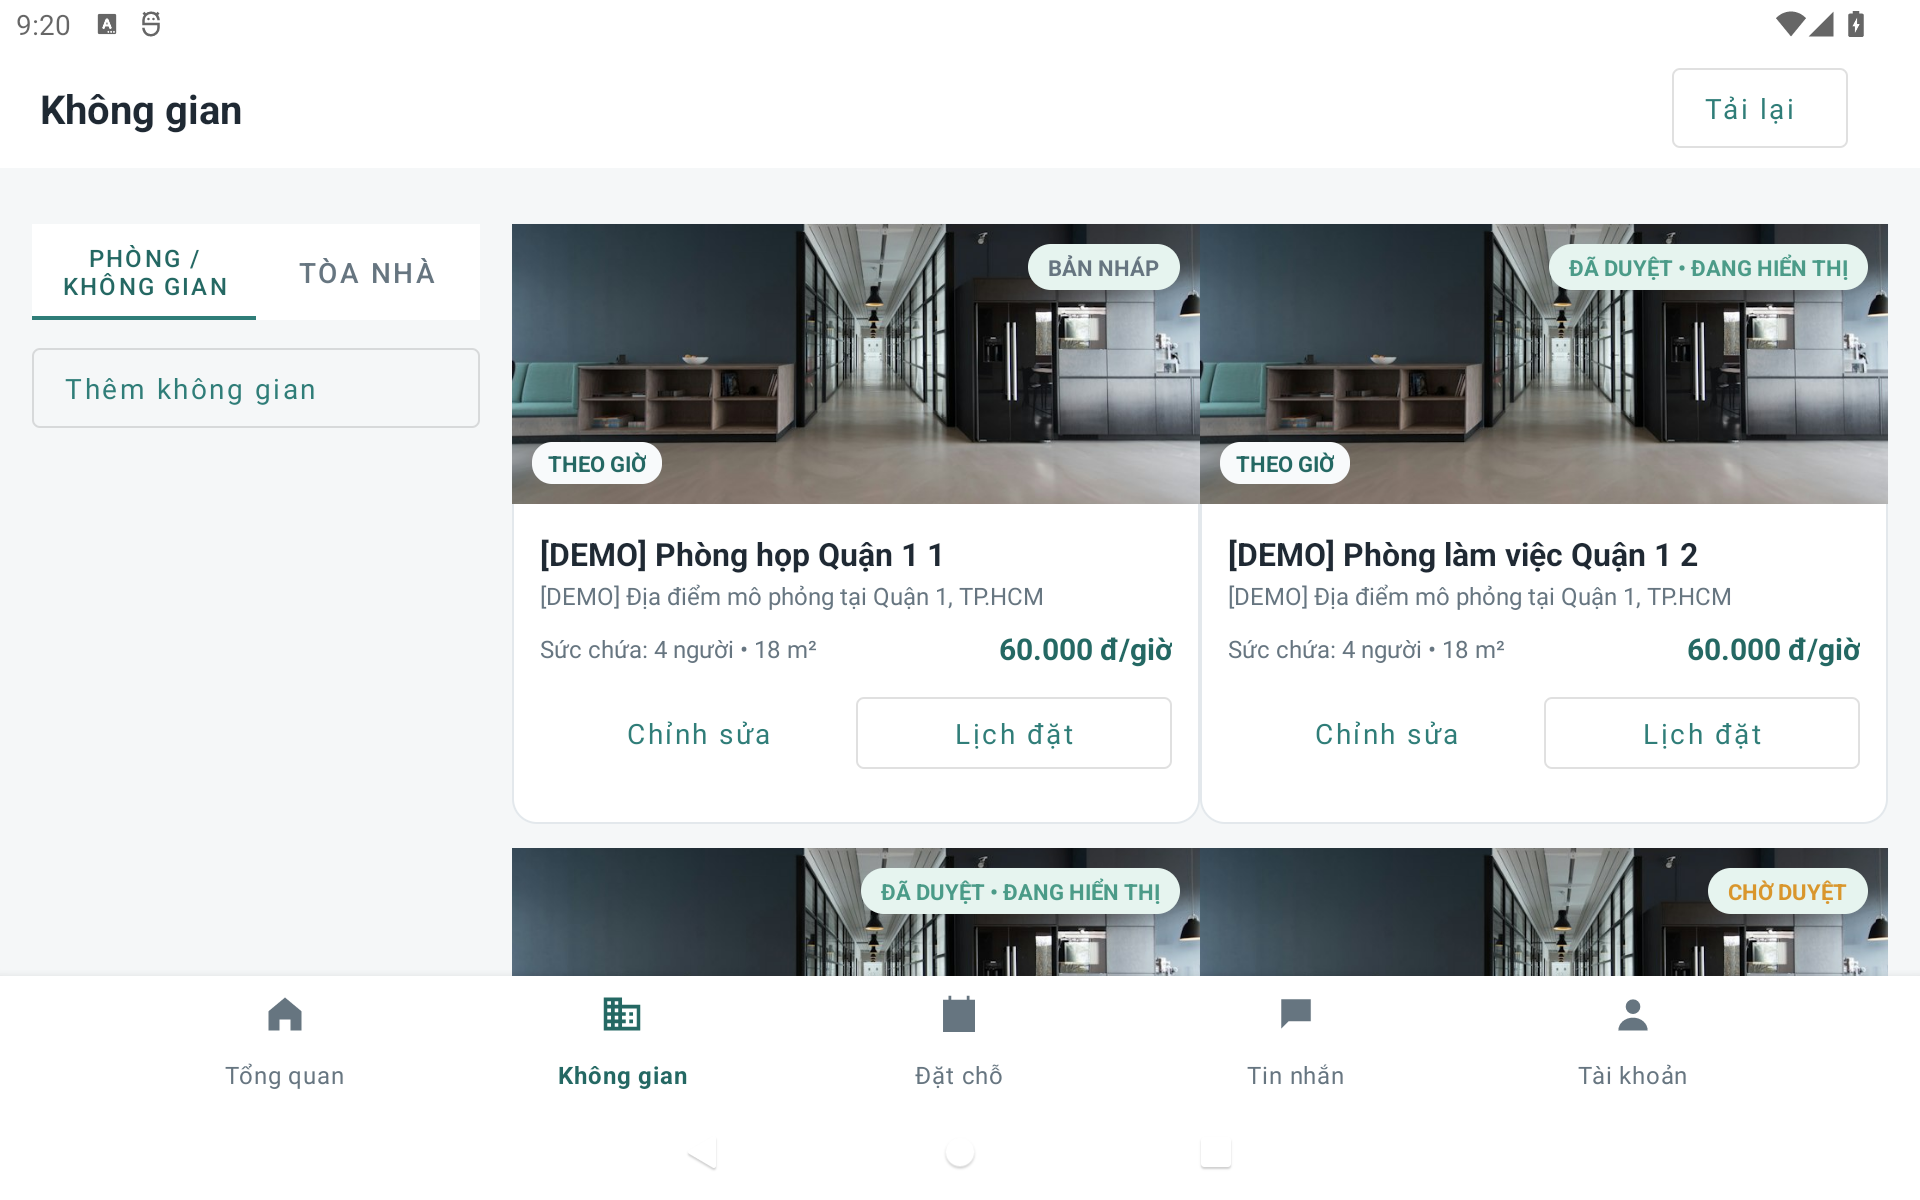
\includegraphics[width=0.94\linewidth]{chapter5/members/host-tablet-spaces-landscape.png}\\[-1mm]
{\small (b) Quản lý không gian của Host}
\caption{Bố cục hai vùng trên tablet Android ở chiều ngang}
\label{fig:adaptive-user-host}
\end{figure}

Activity lưu lựa chọn cần khôi phục, còn ViewModel duy trì dữ liệu qua thay đổi cấu hình \parencite{android_runtime_changes,android_resource_variants}. Khi xoay, tab hoặc bộ lọc đang chọn được phục hồi; màn bản đồ giữ điểm đến và tuyến đã nhận. Listener được quản lý theo vòng đời để tránh đăng ký lặp khi màn hình tái tạo.

\subsubsection{Xử lý trạng thái tải, rỗng, lỗi và quyền truy cập}
Giao diện phân biệt đang tải với danh sách rỗng, khóa thao tác gửi khi request chưa kết thúc và hiển thị lỗi kèm lựa chọn thử lại. Hình~\ref{fig:adaptive-admin} cho thấy kênh Admin đổi cách bố trí theo kích thước: điện thoại ngang giữ tab trên danh sách, tablet ngang đặt nhóm hồ sơ ở cột trái. Quyền xét duyệt vẫn được kiểm tra từ phiên và dữ liệu hiện tại, không thay đổi theo bố cục.

\begin{figure}[H]\centering
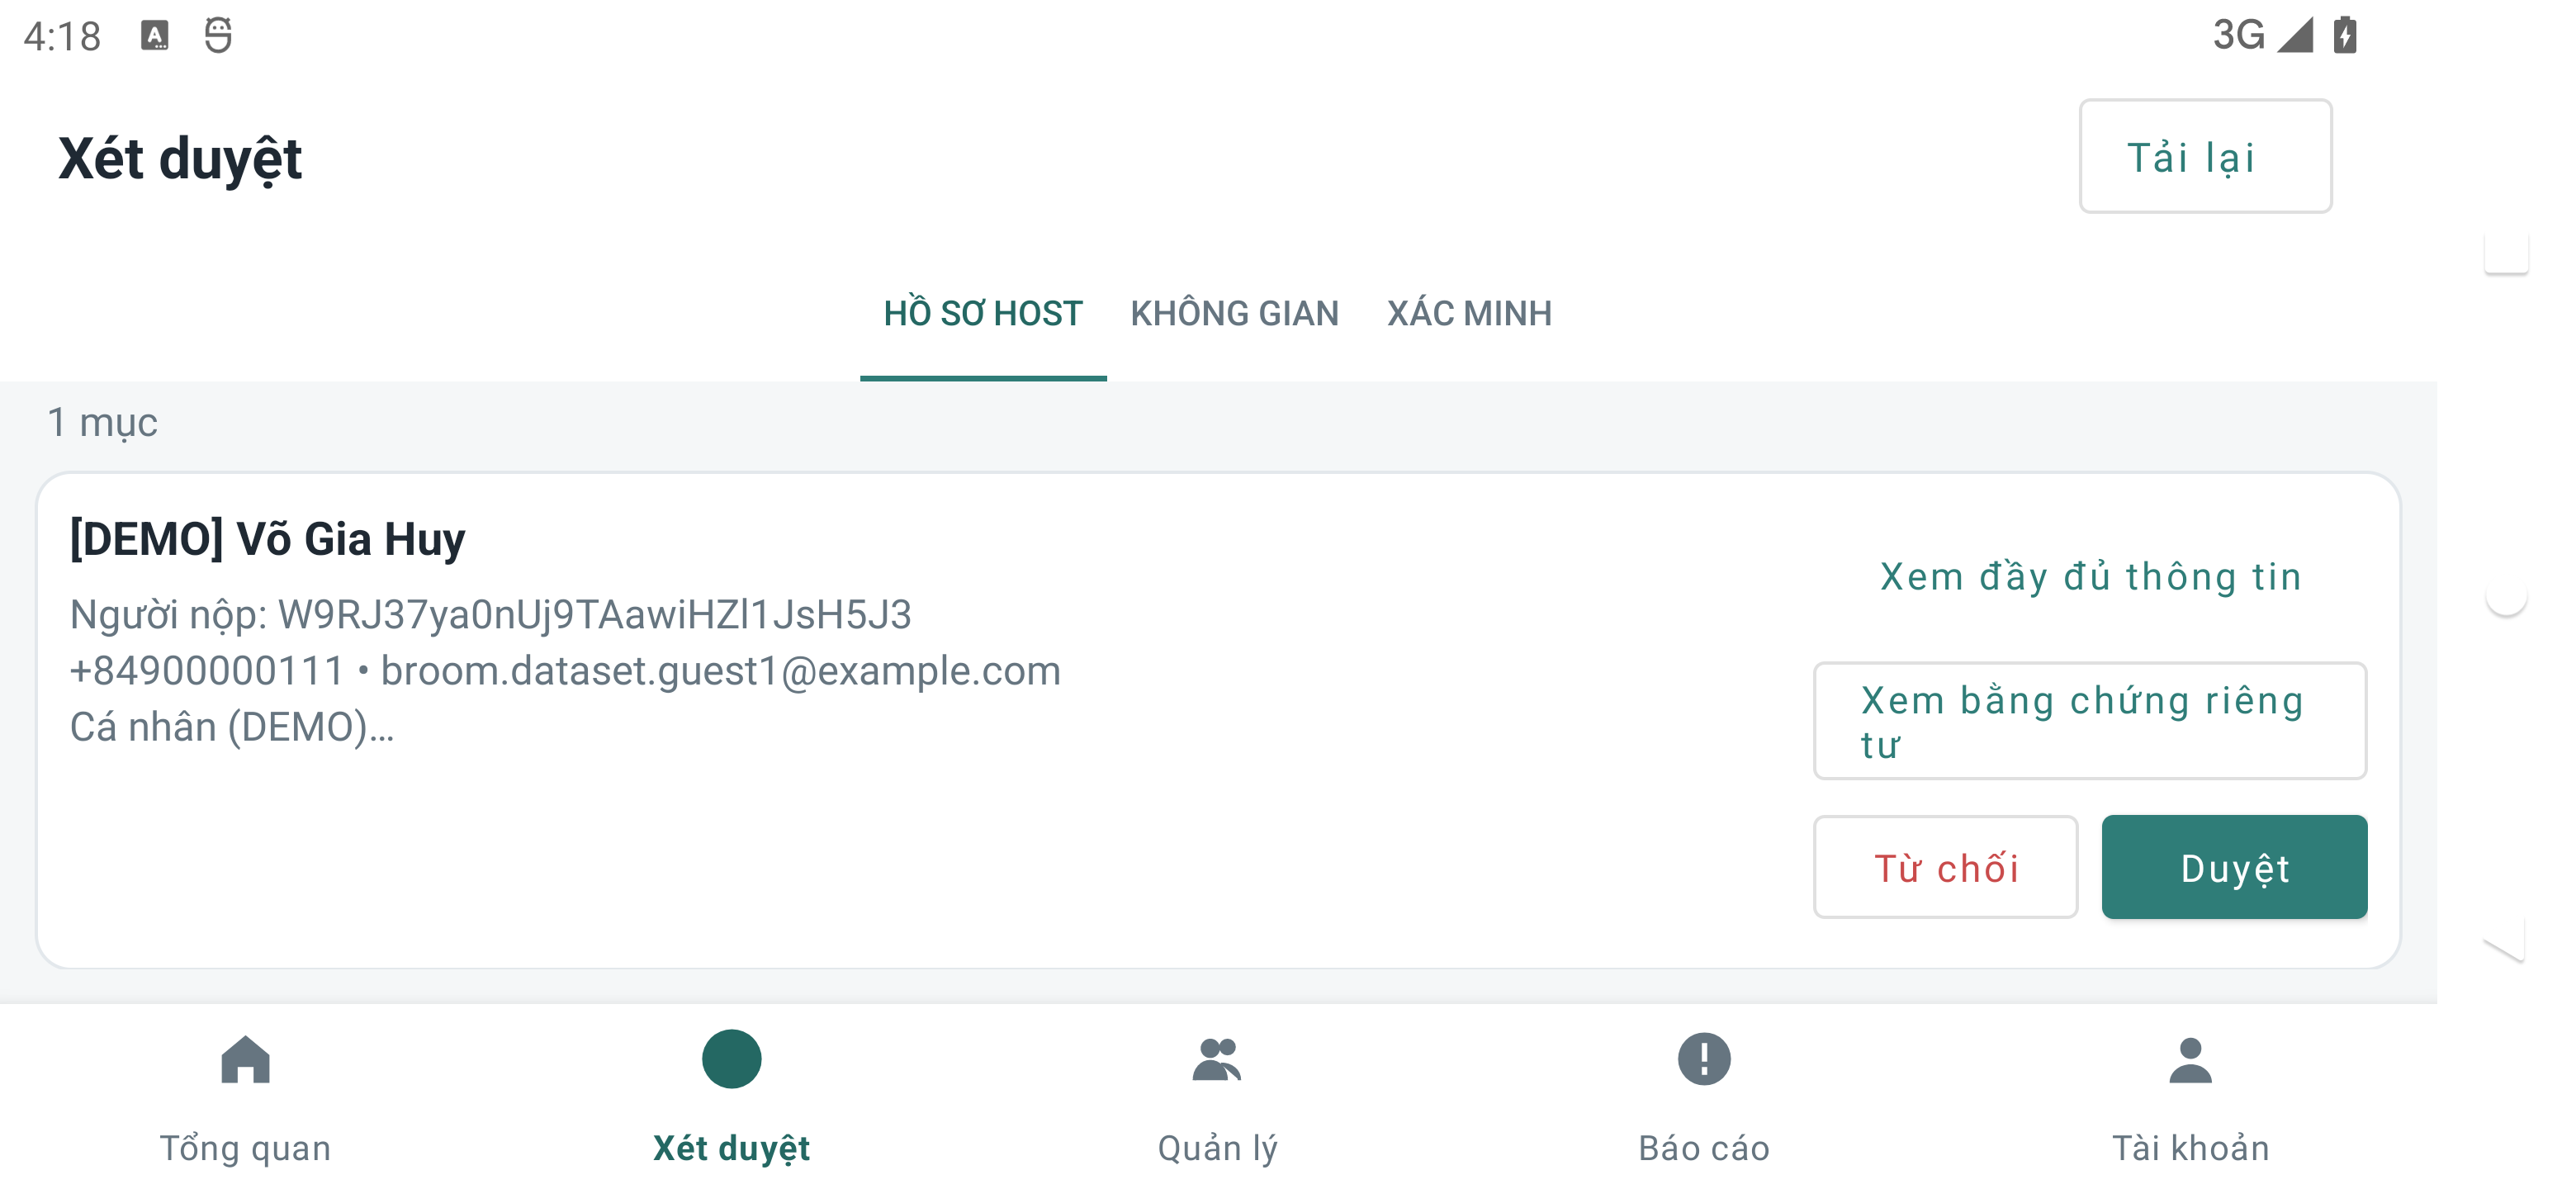
\includegraphics[width=0.94\linewidth]{chapter5/admin-phone-landscape.png}\\[-1mm]
{\small (a) Điện thoại ngang}
\par\medskip
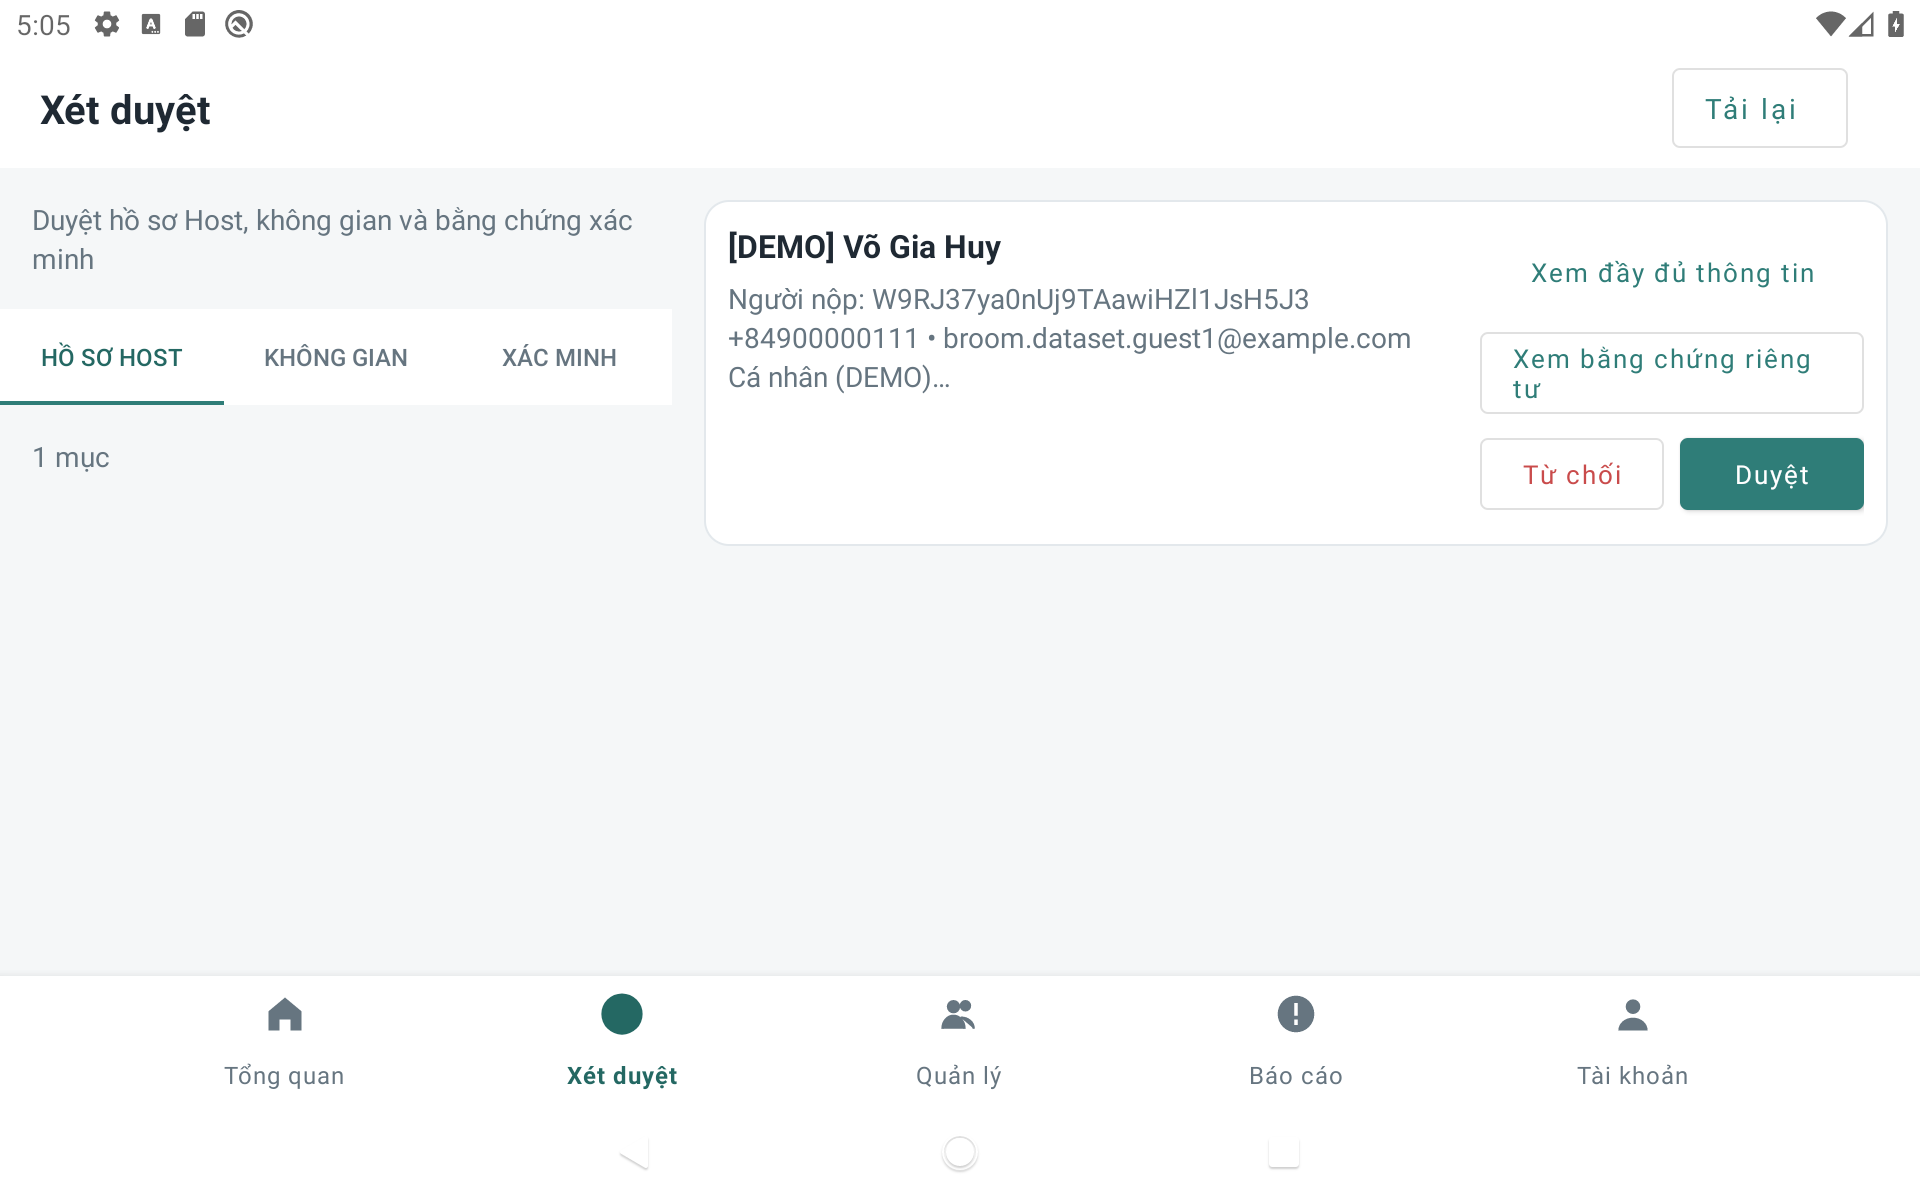
\includegraphics[width=0.94\linewidth]{chapter5/admin-tablet-landscape.png}\\[-1mm]
{\small (b) Tablet ngang}
\caption{Giao diện quản trị theo kích thước thiết bị}
\label{fig:adaptive-admin}
\end{figure}

\clearpage
\subsubsection{Lưu và đọc dữ liệu ngoại tuyến bằng SQLite}
\label{sec:sqlite-offline}
OfflineRepository lưu danh sách, chi tiết phòng và booking của người thuê sau khi tải dữ liệu. OfflineDatabase kế thừa \texttt{SQLiteOpenHelper}, tạo database \texttt{broom\_offline.db} với bảng \texttt{snapshots}. Khóa ghép \texttt{(uid, kind, item\_id)} tách tài khoản, loại bản lưu và đối tượng; \texttt{payload} chứa model đã tuần tự hóa thành dữ liệu nhị phân (BLOB), còn \texttt{saved\_at} ghi thời điểm lưu. Việc đọc, ghi chạy trên luồng nền và trả kết quả về giao diện qua ViewModel \parencite{android_sqlite}.

Hình~\ref{fig:sqlite-offline-screens} thể hiện Trang chủ và lịch sử đặt chỗ khi điện thoại đã ngắt mạng. Danh sách vẫn hiển thị nội dung đã tải, kèm nhãn Ngoại tuyến và thời điểm bản lưu. Người dùng mở được chi tiết phòng hoặc booking; các nút đặt chỗ, thanh toán và cập nhật nghiệp vụ bị khóa. Trang không có bản lưu hiển thị thông báo yêu cầu kết nối mạng để tải dữ liệu.

\begin{figure}[H]\centering
\begin{minipage}[t]{0.32\linewidth}\centering
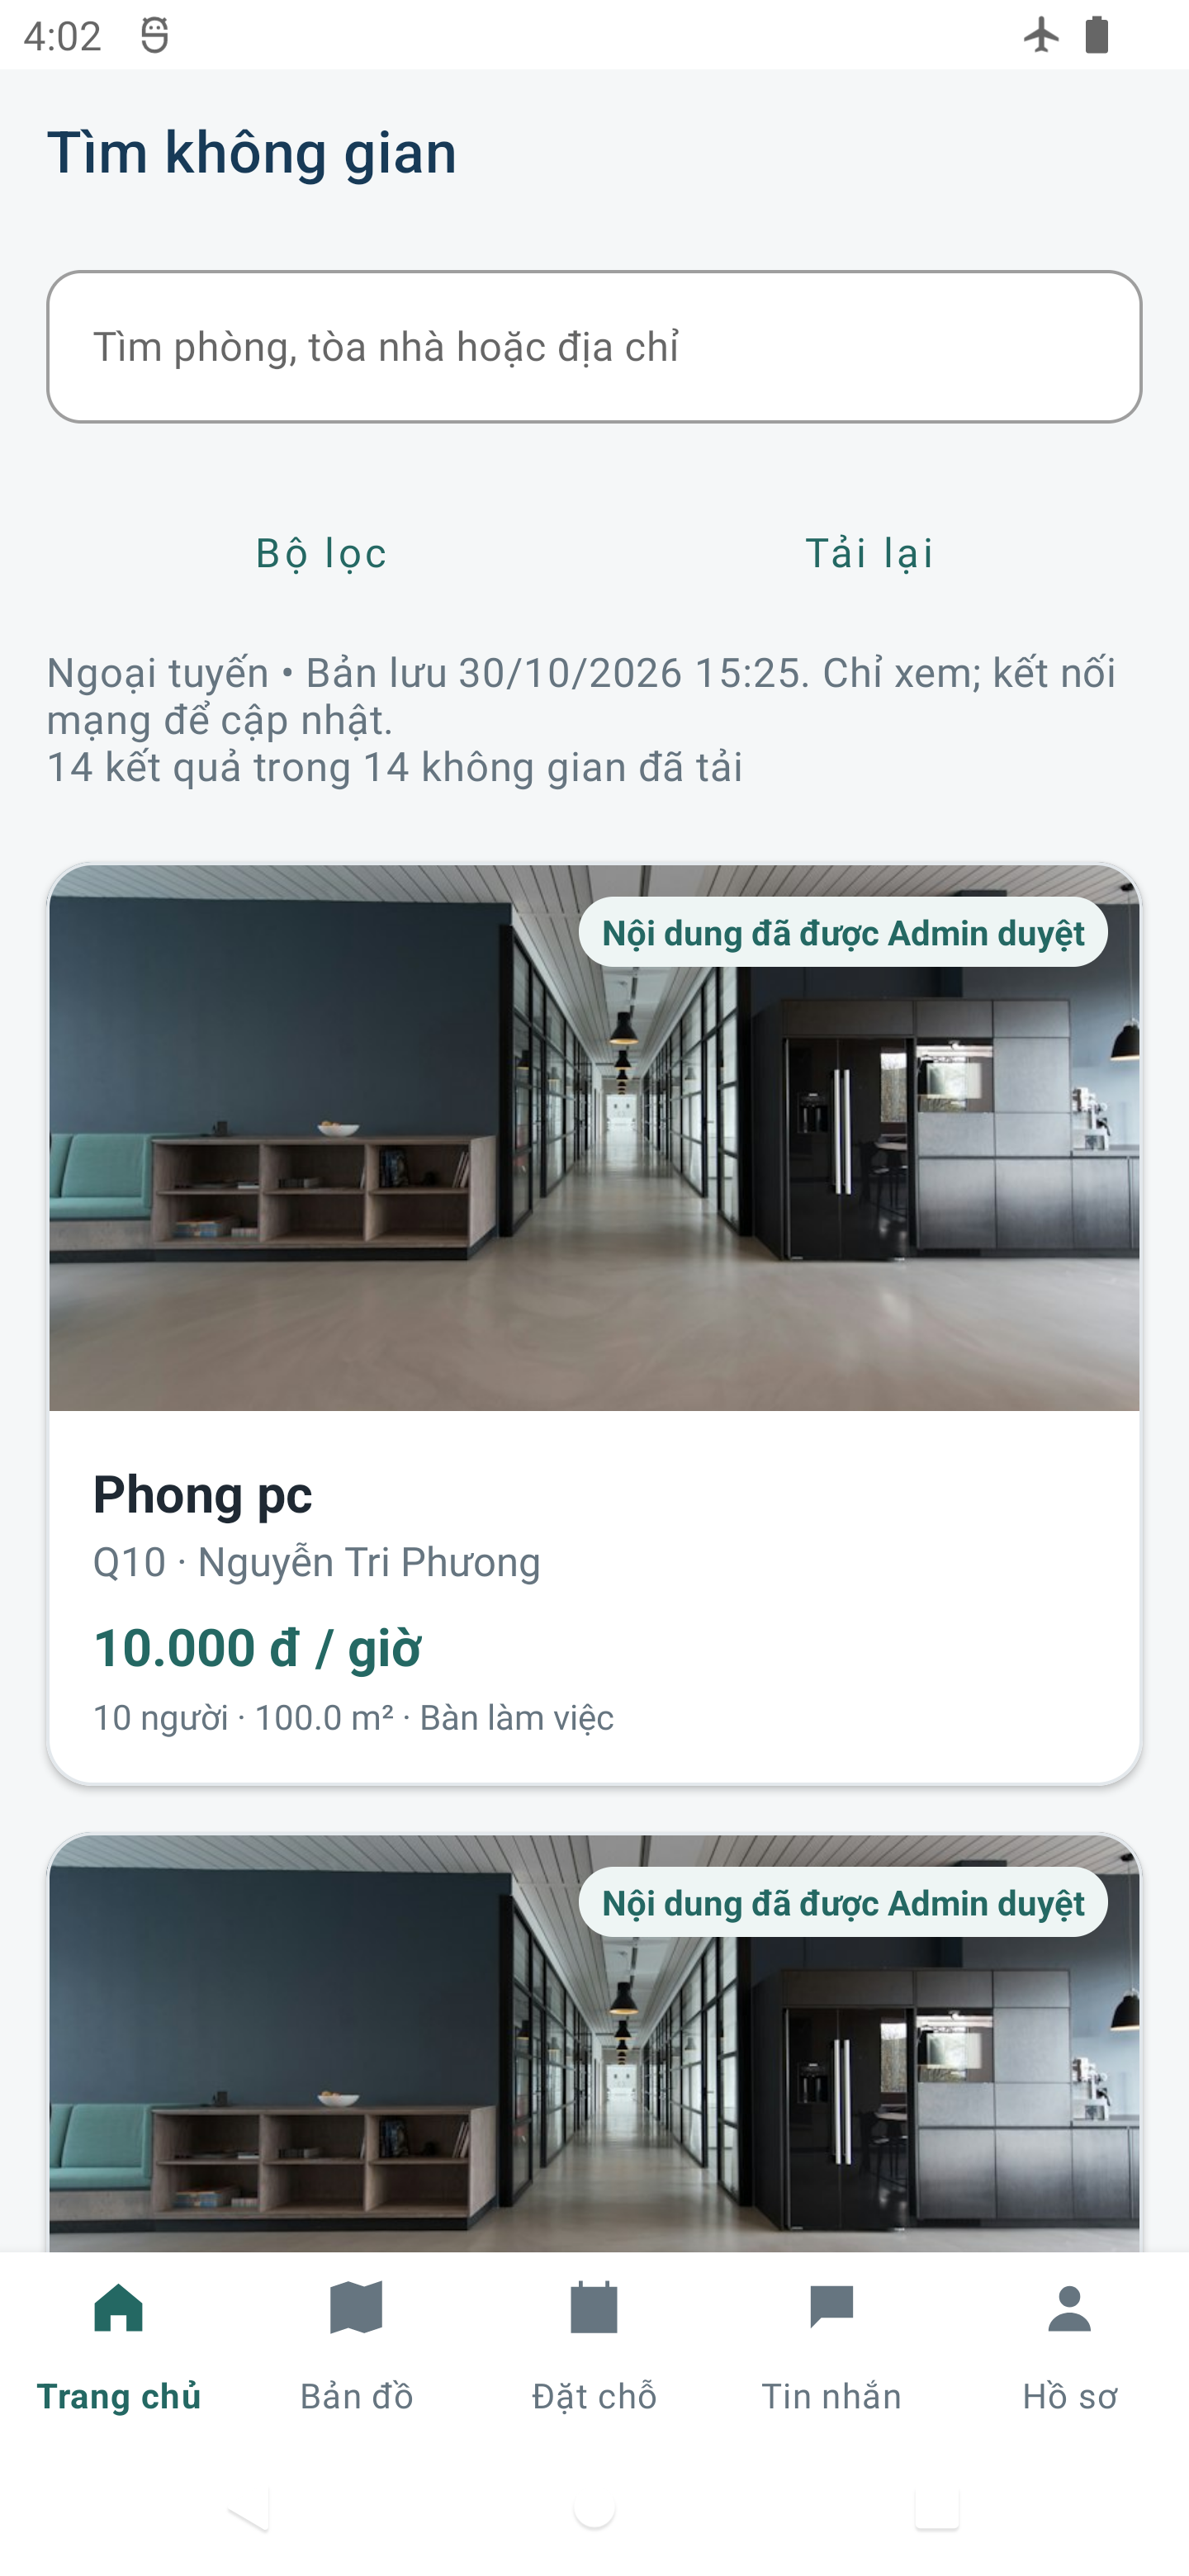
\includegraphics[width=\linewidth]{chapter5/offline/home.png}\\[-1mm]
{\small (a) Phòng đã tải trên Trang chủ}
\end{minipage}\hspace{0.05\linewidth}%
\begin{minipage}[t]{0.32\linewidth}\centering
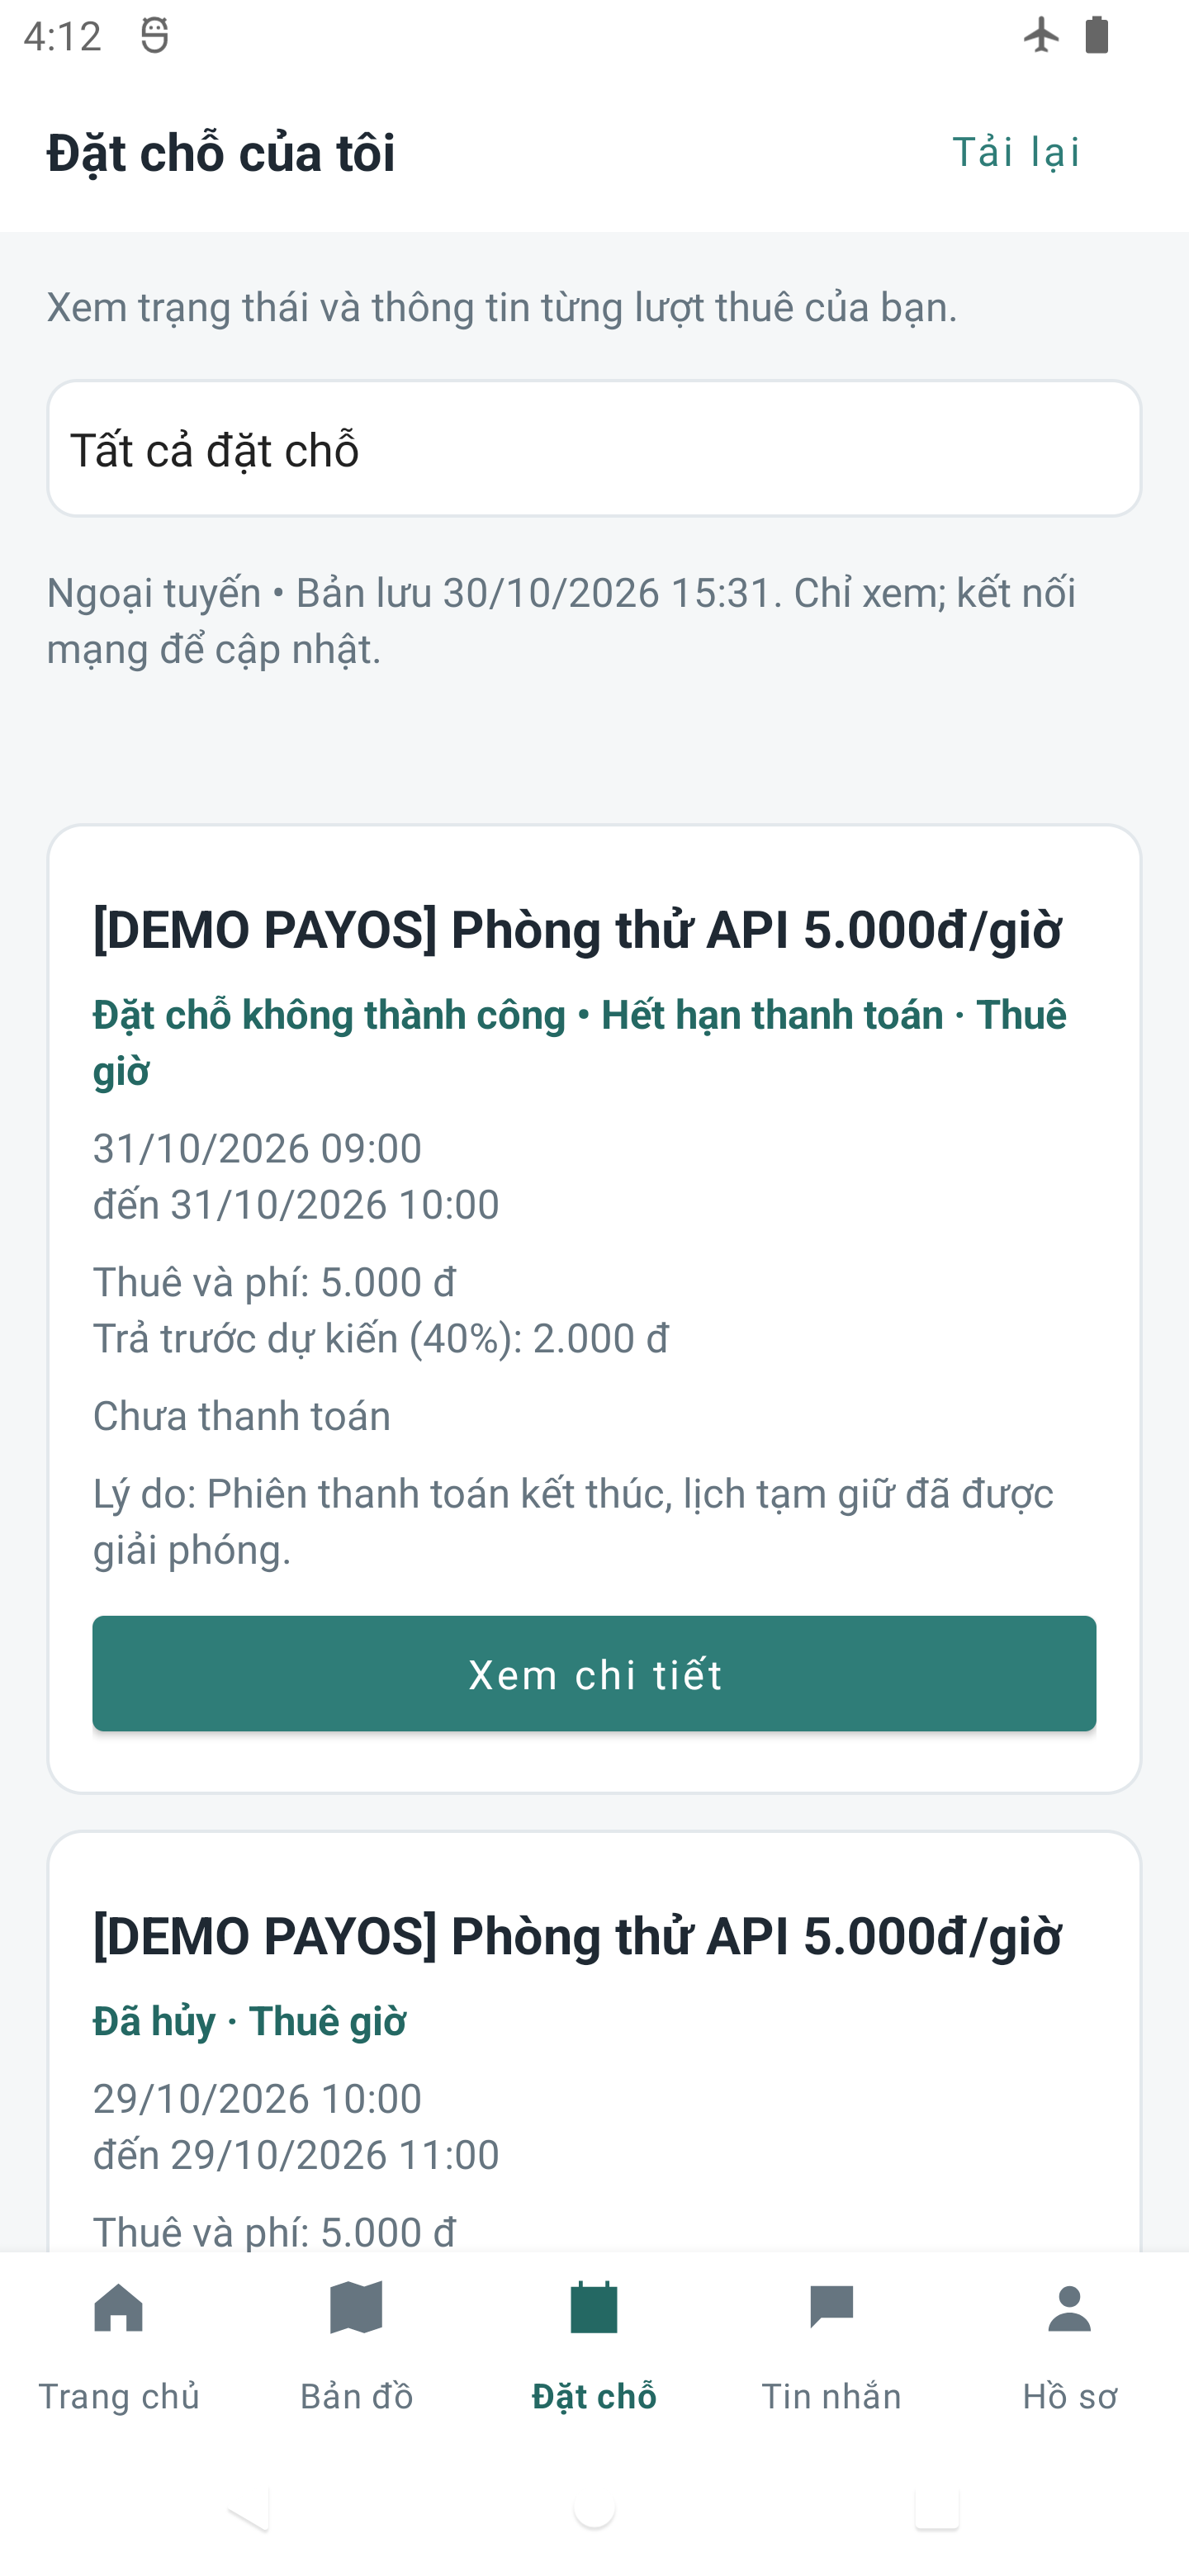
\includegraphics[width=\linewidth]{chapter5/offline/bookings.png}\\[-1mm]
{\small (b) Lịch sử đặt chỗ đã lưu}
\end{minipage}
\caption{Xem dữ liệu từ SQLite khi điện thoại mất kết nối mạng}
\label{fig:sqlite-offline-screens}
\end{figure}

Bản lưu tồn tại sau khi đóng và mở lại ứng dụng. Khi có mạng, SessionActivity kiểm tra phiên và tải dữ liệu hiện tại; lỗi quyền truy cập không được thay bằng kết quả cục bộ. Đăng xuất xóa bản lưu của UID tương ứng. SQLite chỉ lưu dữ liệu để đọc lại, không xếp hàng giao dịch đặt chỗ hoặc thanh toán; ảnh do bộ nhớ đệm của thư viện hiển thị ảnh quản lý riêng.
